% =====================================================================
% APÊNDICE D -- aumento de SNR por configuração, em cada perfil de mobilidade.
% 2026-11-13: texto e figura vieram da seção Mobility profiles (RESULTADOS/formatos.tex);
%   lá ficou só a figura por formato (perfis_mobilidade_formatos). Dados:
%   software/testes/.../figuras/perfis/tcc_perfis_mobilidade_3col_data.csv (figuras_perfis.py).
% =====================================================================

Figure~\ref{fig:perfis-mobilidade} breaks down the largest SNR increase by mobility profile (Section~\ref{subsec:setup_condicoes}). Each point represents the largest increase among the test conditions of a profile. Each row corresponds to a group, and the columns follow the structure of Table~\ref{tab:formatos-escolhidos}: the first two columns include all configurations, the first with the 3~dB format and the second with the 0.1~dB format, while the third column includes only the 10~dB IoTh configurations, with the 3~dB format selected specifically for that subset. When the difference between them exceeds 0.1~dB, the high-mobility profile shows the larger SNR increase (filled point to the right of the unfilled one). The largest observed difference is 0.58~dB, in configuration 2D with $\langle 22,12\rangle$: 0.80~dB for low mobility versus 1.39~dB for high mobility.
% ANTIGO: In all the plots, both mobility profiles meet the criterion of the column. [...] Consequently, the choice of format does not change with the mobility profile.

\begin{figure}[!htb]
\caption{\textcolor{red}{Largest SNR increase, in dB, of each configuration in each mobility profile, in the three groups, with the selected formats.}}
\label{fig:perfis-mobilidade}
\vspace{4pt} % a classe zera o espaço entre a caption e a figura
\centering
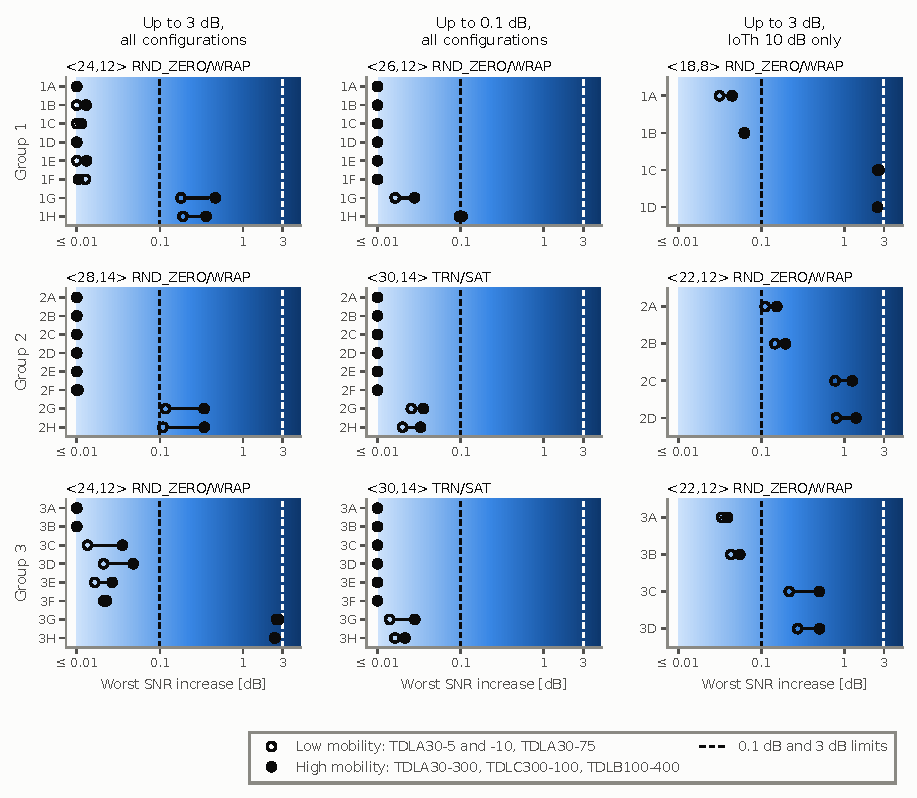
\includegraphics[width=\textwidth]{Images/RESULTADOS/perfis_mobilidade_3col.pdf}
\vspace{4pt}
\legend{\textcolor{red}{Source: the author.}}
\end{figure}
